\documentclass[14pt]{extarticle}
% \documentclass[14pt]{article}

% \usepackage[style=authoryear,maxbibnames=9,maxcitenames=2,uniquelist=false,backend=biber,doi=false,url=false]{biblatex}
% \addbibresource{$BIB} % bibtex location
% \renewcommand*{\nameyeardelim}{\addcomma\space} % have comma in parencite
\usepackage{natbib}

\usepackage{xcolor}
\usepackage{amsmath}
\newcommand{\tuple}[1]{ \langle #1 \rangle }
%\usepackage{automata}
\usepackage{times}
\usepackage{ltablex}
\usepackage{tasks}

%%%%%% Template
\usepackage{hyperref}
\hypersetup{colorlinks=true,allcolors=blue}

\usepackage{vmargin}
\setpapersize{USletter}
\setmarginsrb{1.0in}{1.0in}{1.0in}{0.6in}{0pt}{0pt}{0pt}{0.4in}

% HOW TO USE THE ABOVE:
%\setmarginsrb{leftmargin}{topmargin}{rightmargin}{bottommargin}{headheight}{headsep}{footheight}{footskip}
%\raggedbottom
% paragraphs indent & skip:
\parindent  0.3cm
\parskip    -0.01cm

\usepackage{tikz}
\usetikzlibrary{backgrounds}

% hyphenation:
% \hyphenpenalty=10000 % no hyphen
% \exhyphenpenalty=10000 % no hyphen
\sloppy

% notes-style paragraph spacing and indentation:
\usepackage{parskip}
\setlength{\parindent}{0cm}

% let derivations break across pages
\allowdisplaybreaks

\newcommand{\orange}[1]{\textcolor{orange}{#1}}
\newcommand{\blue}[1]{\textcolor{blue}{#1}}
\newcommand{\red}[1]{\textcolor{red}{#1}}
\newcommand{\freq}[1]{{\bf \sf F}(#1)}
\newcommand{\datafreq}[2]{{{\bf \sf F}_{#1}(#2)}}

\def\qqquad{\quad\qquad}
\def\qqqquad{\qquad\qquad}

%%%%%%%%%%%%%%%%%%%%%%%%%%%%%%%%%%%%%%%%%%%%%%%%%%%%%%%%%%%%%%%%%%%%%%%%%%%%%%%%
%%%%%%%%%%%%%%%%%%%%%%%%%%%%%%%%%%%%%%%%%%%%%%%%%%%%%%%%%%%%%%%%%%%%%%%%%%%%%%%%

% fill-in-blank question style, found in https://tex.stackexchange.com/a/505089

\usepackage{ifthen}
\usepackage{tocloft}
\usepackage{exercise}
% \usepackage{xcolor}

% Set the Show Answers Boolean
\newboolean{showAns}
\setboolean{showAns}{false}
\newcommand{\showAns}{\setboolean{showAns}{true}}

% The length of the Answer line
\newlength{\answerlength}
\newcommand{\anslen}[1]{\settowidth{\answerlength}{#1}}

% ans command that indicates space for an answer or shows the answer in red
\newcommand{\ans}[1]{\settowidth{\answerlength}{\hspace{2ex}#1\hspace{2ex}}%
    \ifthenelse{\boolean{showAns}}%
        {\textcolor{red}{\underline{\hspace{2ex}#1\hspace{2ex}}}}%
        {\underline{\hspace{\answerlength}}}}%

\newcommand{\details}[1]{\settowidth{\answerlength}{#1}%
    \ifthenelse{\boolean{showAns}}%
        {\\ \textcolor{blue}{#1}}%
        {}}%

% Formatting how multiple choices Questions are formated.
\settasks{label=(\Alph*), label-width=30pt}


% Some commands for the Exercise Question package
\renewcommand{\QuestionNB}{\Large\protect\textcircled{\small\bfseries\arabic{Question}}\ }
\renewcommand{\ExerciseHeader}{} %no header
\renewcommand{\QuestionBefore}{3ex} %Space above each Q
\setlength{\QuestionIndent}{8pt} % Indent after Q number


% To create the list of answers with tocloft...
\newcommand{\listanswername}{Answers}
\newlistof[Question]{answer}{Answers}{\listanswername}

% Creates a TOC for Answers
\newcounter{prevQ}
\newcommand{\answer}[1]{\refstepcounter{answer}%
\ans{#1}%
\ifnum\theQuestion=\theprevQ%
        \addcontentsline{Answers}{answer}{\protect\numberline{}#1}% don't include the Q number
        \else%
        \addcontentsline{Answers}{answer}{\protect\numberline{\theQuestion}#1}%
        \setcounter{prevQ}{\value{Question}}%
        \fi%
        }%

% \hyphenpenalty=10000 % no hyphen
% \exhyphenpenalty=10000 % no hyphen
\sloppy              % hyphen

\newcommand{\HRule}{\rule{\linewidth}{0.5mm}}
\newcommand{\Hrule}{\rule{\linewidth}{0.3mm}}

%tocloft formatting listofanswers
\renewcommand{\cftAnswerstitlefont}{\bfseries\large}
\renewcommand{\cftanswerdotsep}{\cftnodots}
\cftpagenumbersoff{answer}
\addtolength{\cftanswernumwidth}{10pt}

\makeatletter% since there's an at-sign (@) in the command name
\renewcommand{\@maketitle}{%
  \parindent=0pt% don't indent paragraphs in the title block
  \centering
  {\Large \bfseries\textsc{\@title}} \\
  \vspace{5pt}
  {\large \textit{\@author}} \\
  \HRule \\
  \vspace{1em}
}
\makeatother% resets the meaning of the at-sign (@)

\title{ECON 2002.01 Problem Set 8 }
\author{Unit 14 \\
  \vspace{5pt}
    Hui-Jun Chen}


%%%%%%%%%%%%%%%%%%%%%%%%%%%%%%%%%%%%%%%%%%%%%%%%%%%%%%%%%%%%%%%%%%%%%%%%%%%%%%%%
%%%%%%%%%%%%%%%%%%%%%%%%%%%%%%%%%%%%%%%%%%%%%%%%%%%%%%%%%%%%%%%%%%%%%%%%%%%%%%%%
\begin{document}

\maketitle

\showAns
\listofanswer

    % 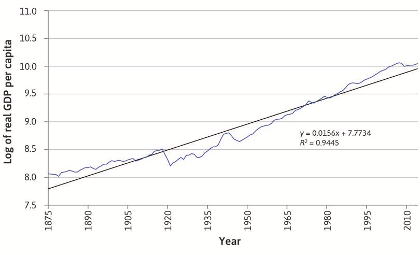
\includegraphics[width=\textwidth]{../QuestionBankImage/OUP-U13-Q04-01.png}

\begin{Exercise}

\Question (OUP-U14-Q3)
In the expression for aggregate consumption $C = C_0 + C_1 Y$, $ C_1 $ is known as:
\answer{D}
\begin{tasks}(1)
    \task Autonomous consumption.
        \details{‘Autonomous’ means independent of income. $ C_0 $ shows the level of consumption that does not depend upon income.}
    \task The average propensity to consume.
        \details{The average propensity to consume is given by total consumption divided by income. $ C_1 $ shows the extent to which consumption changes with income. Assuming that $ C_1 $ is less than one, the average propensity to consume will be falling as income increases even though $ C_1 $ is constant.}
    \task The multiplier.
        \details{The multiplier shows the extent to which income changes as a result of a change in autonomous spending. The formula for the (simple) multiplier is $1/(1 - C_1)$.}
    \task The marginal propensity to consume.
        \details{$ C_1 $ is the marginal propensity to consume. It normally take a value less than one, showing that an initial change in autonomous spending will initiate a series of changes of diminishing size.}
\end{tasks}



\Question (OUP-U14-Q7)
In an economy with no taxation and no external trade, the size of the multiplier depends on:
\answer{D}
\begin{tasks}(1)
    \task Investment.
        \details{In a closed economy with no government, the level of investment determines the current level of aggregate demand ($Y = C + I$).}
    \task The current level of aggregate demand.
        \details{The simple multiplier formula is $1/(1 - MPC)$, which does not depend on the level of aggregate demand ($ Y $).}
    \task Autonomous consumption.
        \details{Autonomous consumption ($ C_0 $) is the part of consumption that does not depend upon income, so it would not affect the size of the multiplier.}
    \task The marginal propensity to consume.
        \details{The simple multiplier formula is $1/(1 - MPC)$, where MPC is the marginal propensity to consume.}
\end{tasks}



\Question (OUP-U14-Q10)
In the figure shown, a fall in output is caused by a reduction in investment. Which of the following would help restore output to its original level?

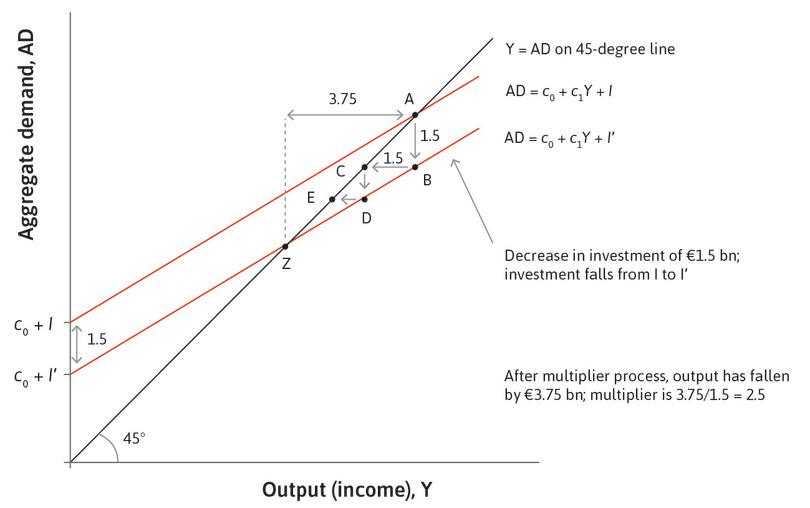
\includegraphics[width=\textwidth]{../QuestionBankImage/OUP-U14-Q10-01.jpg}
\answer{C}
\begin{tasks}(1)
    \task A reduction in autonomous consumption.
        \details{What is required is some compensating increase in aggregate demand. A reduction in autonomous consumption (the vertical axis intercept) will further reduce aggregate demand.}
    \task An increase in target wealth.
        \details{An increase in target wealth is likely to encourage households to save more, thus reducing aggregate demand.}
    \task An increase in actual wealth.
        \details{However, an increase in actual wealth may persuade them that there is less need to save. If so, consumption will increase and may compensate for the fall in investment.}
    \task A tightening of credit conditions.
        \details{A tightening of credit conditions will make borrowing more difficult, which will discourage consumption and may also encourage saving (which will also reduce consumption).}
\end{tasks}



\Question (OUP-U14-Q12)
In an economy where the MPC is 0.7, the proportional tax rate is 0.25 and the marginal propensity to import is 0.2, the multiplier will be:

\textit{Hint:} There's both MPC, proportional tax rate and MPI needs to be considered
\answer{C}
\begin{tasks}(1)
    \task 0.675
        \details{The value of the multiplier in this case is: 1/(1 - 0.7(0.75)) + 0.2 = 1/(1 - 0.525) + 0.2 = 1.48. 0.675 is the value of the multiplier if we omit the 1 in the numerator i.e. 0.475 + 0.2.}
    \task 2.1
        \details{The value of the multiplier in this case is: 1/(1 - 0.7(0.75)) + 0.2 = 1/(1 - 0.525) + 0.2 = 1.48. 2.1 is the value of the multiplier if we omit the marginal propensity to import.}
    \task 1.48
        \details{The value of the multiplier in this case is: 1/(1 - 0.7(0.75)) + 0.2 = 1/(1 - 0.525) + 0.2 = 1.48.}
    \task 2.35
        \details{The value of the multiplier in this case is: 1/(1 - 0.7(0.75)) + 0.2 = 1/(1 - 0.525) + 0.2 = 1.48. 2.35 is the value of the multiplier if we do the calculations in the wrong order, i.e. (1 - 0.7)0.75 + 0.2.}
\end{tasks}



\Question (OUP-U14-Q15)
The central bank announces a rise in the official interest rate to reduce the rate of inflation. Looking at the figure shown, ceteris paribus, the aggregate investment function in these circumstances is likely to:

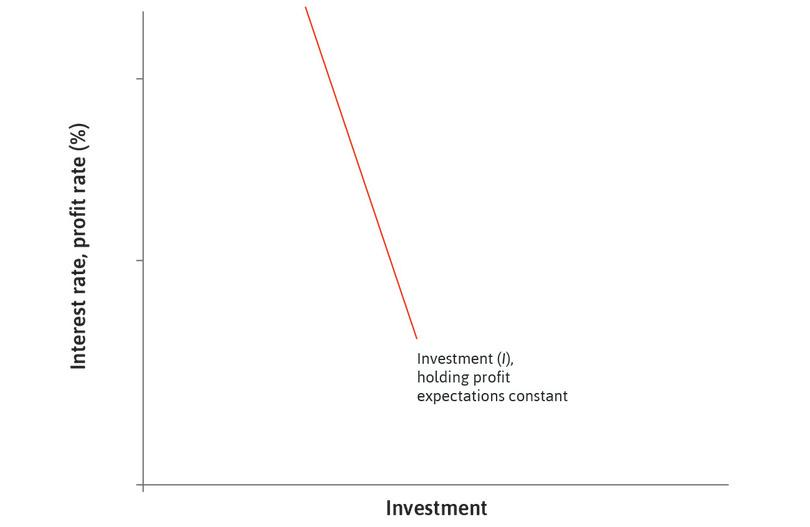
\includegraphics[width=\textwidth]{../QuestionBankImage/OUP-U14-Q15-01.jpg}
\answer{D}
\begin{tasks}(1)
    \task Become flatter.
        \details{The aggregate investment function shows the relationship between investment spending and the interest rate, ceteris paribus. A rise in the official interest rate moves us up along the investment function, indicating a fall in investment. There is no need for the investment function itself to change.}
    \task Become steeper.
        \details{Because we are dealing with a change in a variable on one of the axes, there is no need for the function itself to change. This will happen only if there is a change in some other relevant variable, not shown in the diagram.}
    \task Shift to the left.
        \details{Because we are dealing with a change in a variable on one of the axes, there is no need for the function itself to change. This will happen only if there is a change in some other relevant variable, not shown in the diagram.}
    \task Remain unchanged.
        \details{A rise in the official interest rate moves us up along the investment function, indicating a fall in investment. There is no need for the investment function itself to change.}
\end{tasks}



\Question (OUP-U14-Q22)
Cuts in public expenditure do not guarantee a reduction in the government’s deficit because:
\answer{B}
\begin{tasks}(1)
    \task Firms will try to pay less tax.
        \details{Firms (and households) may try to minimise their tax liabilities, but there is no reason to suppose that their attempts to do this are directly related to the level of government spending.}
    \task Aggregate demand will fall, reducing government revenue.
        \details{The cuts in public spending constitute a reduction in the autonomous components of aggregate demand. Through the multiplier, we must expect a fall in aggregate demand somewhat larger than the initial cut in public spending. With the fall in aggregate demand, output, and employment, there will be a fall in government revenue as fewer workers pay tax and firms pay less tax on their lower profits.}
    \task Aggregate demand falls, and firms invest less.
        \details{Aggregate demand will fall and firms may decide to invest less if they see this reduction in aggregate demand as a condition that is likely to persist, but the reduction in investment has no direct connection to the government’s revenue.}
    \task There is a fall in autonomous consumption.
        \details{There is no reason to expect a fall in autonomous consumption. Aggregate demand will fall, meaning that income will fall and there may be some reduction in consumer spending (the basis of the multiplier effect). But this will be consumer spending that is related to income, not autonomous consumption ($ C_1 $ not $ C_0 $).}
\end{tasks}


\Question (OUP-U14-Q24)
In an economy with unutilised resources, the government stimulates aggregate demand by increasing its spending. The effect on output and employment will be greater if:
\answer{C}
\begin{tasks}(1)
    \task The economy has a high propensity to import.
        \details{If the economy has a high propensity to import, a stimulus to aggregate demand will result in an increase in imports. This reduces any subsequent additions to aggregate demand through the multiplier (i.e. the multiplier is smaller).}
    \task The spending is financed by additional taxation.
        \details{Taxation is a ‘leakage’ from the circular flow of income and an increase therefore reduces aggregate demand. If the spending is financed by additional taxation, the additional taxation will at least partly offset the expansionary effect of the spending.}
    \task Its trading partners undertake a similar policy.
        \details{The stimulus to aggregate demand in country A will be reinforced if the trading partners also adopt expansionary policies. This is because their expanding economies will require more imports and some of those will be exports from country A. This increase in exports constitutes a further addition to aggregate demand in country A.}
    \task The central bank simultaneously tightens monetary policy.
        \details{If the central bank tightens monetary policy this will have a negative effect on investment and on some consumer spending. It will tend to offset the fiscal stimulus. By contrast, a loosening of monetary policy would reinforce the increase in government spending.}
\end{tasks}




\Question (OUP-U14-Q11)
A multiplier of 3 or above would be considered exceptionally high for most modern economies. Which of the following statements gives the most complete explanation for this fact?
\answer{D}
\begin{tasks}(1)
    \task The national accounts overstate consumption.
        \details{Simply overstating consumption would not be enough to produce an exaggerated value for the multiplier, which depends on the MPC. The accounts would have to show us that the MPC were larger than it actually is.}
    \task Credit is probably easier to obtain than we think.
        \details{If this were true, then it would tend to diminish our calculation of the multiplier since access to credit enables households to smooth the effect of income fluctuations, and this reduces the size of the multiplier.}
    \task We have overlooked the effect of taxation.
        \details{Taxation is an additional ‘leakage’ from the circular flow of income. It affects the multiplier in a similar way to saving. So omitting the effect of taxation will yield an unrealistically high value for the multiplier – but may not be the whole story.}
    \task We have overlooked the effect of taxation and external trade.
        \details{Imports also represent a ‘leakage’ and affect the multiplier in the same way as saving and taxation. Since all real world economies involve government and overseas trade, we need a formula for the multiplier including the marginal rate of tax ($ t $) and the propensity to import ($ m $). This is: $1/(1 - MPC x (1 - t)) + m$.}
\end{tasks}



\Question (OUP-U14-Q16)
The figure shows a downward shift of the aggregate demand curve, reducing the level of output from A to Z. Suppose that we begin again at A and that this is a full-employment level of output. An increase in aggregate demand in these circumstances will most likely cause:

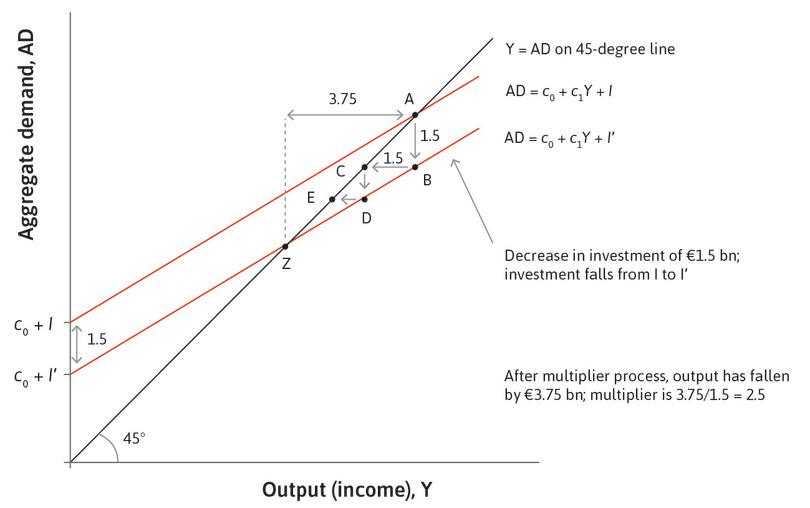
\includegraphics[width=\textwidth]{../QuestionBankImage/OUP-U14-Q10-01.jpg}
\answer{D}

\begin{tasks}(1)
    \task An increase in employment.
        \details{If the economy is producing a full employment level of output, an increase in aggregate demand cannot create more employment. It may create more jobs in one industry at the expense of another as firms compete with each other to attract more workers, but there cannot be an overall increase in employment.}
    \task A fall in wages.
        \details{The increase in aggregate demand will probably cause firms to compete against each other in a self-defeating attempt to attract more workers. This will involve higher nominal wages, but the real wage will be unchanged as firms raise prices to cover the higher nominal wages.}
    \task An increase in output.
        \details{At full employment, an increase in aggregate demand cannot produce additional output.}
    \task A rise in the general level of prices.
        \details{Attempts to increase aggregate demand when the economy is already at full employment will almost certainly cause a rise in the general price level.}
\end{tasks}



\Question (OUP-U14-Q18)
The ‘paradox of thrift’ refers to the fact that:
\answer{A}
\begin{tasks}(1)
    \task If we all save more, aggregate income will fall.
        \details{If an individual reduces his/her consumption in order to save more, he/she will usually be successful. But if we all save more, this reduces the level of aggregate demand. This in turn will reduce the level of employment and total income. Since saving (and consumption) depend upon the level of income, the fall in income will reduce the total level of saving. Hence a general attempt to save more leads to the paradox that less actual saving takes place.}
    \task The wealthier I become, the more tax I have to pay.
        \details{One objection to taxes on wealth is that it penalises saving. But there is no paradox here.}
    \task Saving is a waste of time.
        \details{Saving, like consumption, is a matter of taste or preference. Some individuals will rate it highly, while others will think it is not worthwhile, especially if interest rates are low. But there is no paradox involved.}
    \task Inflation erodes the value of savings.
        \details{Inflation will erode the value of savings if the rate of inflation exceeds the return on savings. High rates of inflation are sometimes given to justify the view that saving is a waste of time. But this is simply a matter of judgement. No paradox is involved.}
\end{tasks}
\end{Exercise}

\end{document}
